\documentclass[class=article, crop=false]{standalone}
\usepackage{mathtools}
\usepackage{amsmath}
\usepackage{import}
\usepackage{float}
\setcounter{section}{0}
\begin{document}
\section{Introduction}
Les heuristiques sont des méthodes spécifiques qui exploitent au mieux la structure du 
problème dans le but de trouver une solution raisonnable (non nécessairement optimale) en un temps réduit. 
L’utilisation de ce type d’algorithmes s'impose car les méthodes de résolution exactes sont 
de complexité exponentielle, et échouent à trouver la solution pour des instances de tailles moyennes voir petites,
 comme on la constater lors du chapitre précédant . 
L'usage des heuristiques est donc pertinent pour surmonter ces limites.\\

Dans ce chapitre, nous allons présenter la conception détaillée des heuristiques sur lesquelles notre choix d’implémentation s’est porté et qui sont:
\begin{enumerate}
    \item Next Fit (NF)
    \item Next Fit Decreasing (NFD)
    \item First Fit (FF)
    \item First Fit Descreasing (FFD)
    \item Best Fit (BF)
    \item Best Fit Decreasing (BFD)\\
\end{enumerate}

Dans le but d’explorer ces méthodes, comparer leurs performances, montrer leurs avantages et découvrir leurs limites , nous effectuerons des tests empiriques et comparatifs sur les mêmes  benchmarks utilisés pour les tests des méthodes exactes.( Benchmark Scholl)
\newpage
\section{Next Fit (NF)}
\subsection{principe}
Si l’article tient dans la même boite que l’article précédent, il est placé avec ce dernier. Sinon, on ouvre une nouvelle boite et le mettre là-dedans.
\begin{itemize}
    \item NF est un algorithme simple d’une complexité de O(n). 
\end{itemize}

\subsection{Pseudo-Code}
\begin{algorithm}[H]
    \caption{Next Fit}
    \begin{algorithmic}
    \FOR{Tous les articles i = 1, 2,. . . , n}
        \IF{l'article i s'inscrit dans la boîte actuelle}
            \STATE Ranger l’article i dans la boîte actuelle
        \ELSE 
            \STATE Créer une nouvelle boîte, en faire la boîte actuelle et ranger l'article i dedant.
        \ENDIF
    \ENDFOR
    \end{algorithmic}
\end{algorithm}

\section{Next Fit Decreasing (NFD)}
\subsection{principe}
Le NFD est une amélioration de l’algorithme Next-Fit. Cet algorithme ordonne es articles par
 ordre décroissant des poids,puis applique l’algorithme NF.

\subsection{Pseudo-Code}
\begin{algorithm}
    \caption{Next Fit Decreasing }
    \begin{algorithmic}
        \STATE Triez les articles par ordre décroissant
        \STATE Appliquer Next-Fit à la liste triée
    \end{algorithmic}
\end{algorithm}

\begin{figure}[H]
    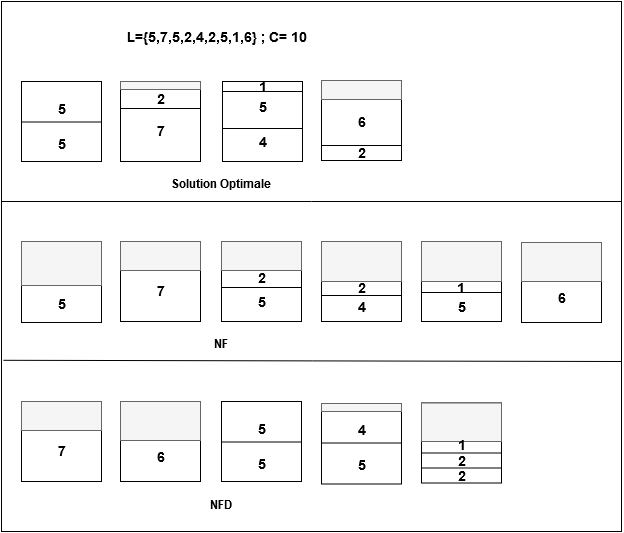
\includegraphics[width=\linewidth]{../figures/NF NFD better(1).png}
    \caption{Exemple NF et NFD}
\end{figure}
\section{First Fit (FF)}
\subsection{principe}
Ranger chaque article courant dans la première boîte, entre celles déjà ouvertes, qui peut le contenir sinon ouvrir une nouvelle boîte et on le range dedans.
\begin{itemize}
    \item L’algorithme First Fit peut être implémenté en O(nlog n ) en utilisant les arbres de recherche binaires
\end{itemize}

\subsection{Pseudo-Code}
\begin{algorithm}[H]
    \caption{First Fit}
    \begin{algorithmic}
    \FOR{Tous les articles i = 1, 2,. . . , n}
        \FOR{Tous les boîtes j = 1, 2,. . . m}
            \IF{l'article i s'inscrit dans la boîte j}
              \STATE Ranger l’article i dans la boîte j
              \STATE Quitter la boucle ( passer à l'article suivant)
             \ENDIF 
        \ENDFOR
        \IF{l’article i ne rentre dans aucune boîte disponible}
            \STATE Créer une nouvelle boîte et ranger l’article i dedans
        \ENDIF
    \ENDFOR
    \end{algorithmic}
\end{algorithm}

\section{First Fit Descreasing (FFD)}
\subsection{principe}
Le FFD est une amélioration de l’algorithme First-Fit . Cet algorithme ordonne les poids dans le sens décroissant puis lui applique l’algorithme FF.
\begin{itemize}
    \item L’algorithme First Fit peut être implémenté en O(nlog n ) en utilisant les arbres de recherche binaires 
\end{itemize}

\subsection{Pseudo-Code}
\begin{algorithm}
    \caption{First Fit Decreasing }
    \begin{algorithmic}
        \STATE Triez les articles par ordre décroissant
        \STATE Appliquer First-Fit à la liste triée 
    \end{algorithmic}
\end{algorithm}

\begin{figure}[H]
    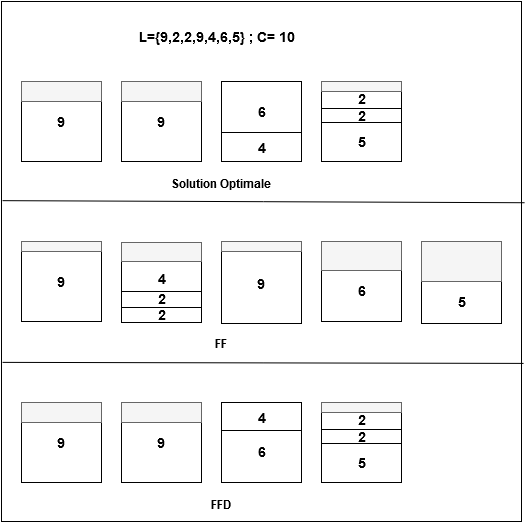
\includegraphics[width=\linewidth]{../figures/FF FFD.png}
    \caption{Exemple FF et FFD}
\end{figure}

\section{Best Fit (BF)}
\subsection{principe}
Ranger chaque article courant dans la boîte la mieux remplie, entre celles déjà ouvertes, qui peut le contenir sinon ouvrir une nouvelle boîte et on le range dedans.
\begin{itemize}
    \item L’algorithme Best Fit peut être implémenté en O(nlog n ) en utilisant les arbres de recherche binaires
\end{itemize}

\subsection{Pseudo-Code}
\begin{algorithm}[H]
    \caption{Best Fit}
    \begin{algorithmic}
    \FOR{Tous les articles i = 1, 2,. . . , n}
        \FOR{Tous les boîtes j = 1, 2,. . . m}
            \IF{l'article i s'inscrit dans la boîte j}
              \STATE Calculer la capacité restante dans la boîte j une fois l'article
             \ENDIF 
        \ENDFOR
        \STATE Ranger l’article i dans la boîte j, où j est la boîte ayant la capacité restante minimale après avoir ajouté l’article(c'est-à-dire que "l’article convient le mieux").
        \IF{une telle boîte n'existe pas ( l’article ne peut être rangé dans aucune boîte)}
            \STATE Créer une nouvelle boîte et ranger l’article i dedans
        \ENDIF
    \ENDFOR
    \end{algorithmic}
\end{algorithm}

\section{Best Fit Decreasing (BFD)}
\subsection{principe}
Le BFD est une amélioration de l’algorithme Best-Fit . Cet algorithme ordonne les poids dans le sens décroissant puis applique l’algorithme BF.

\subsection{Pseudo-Code}

\begin{algorithm}
    \caption{Best Fit Decreasing }
    \begin{algorithmic}
        \STATE Triez les articles par ordre décroissant
        \STATE Appliquer Best-Fit à la liste triée 
    \end{algorithmic}
\end{algorithm}


\begin{figure}[H]
    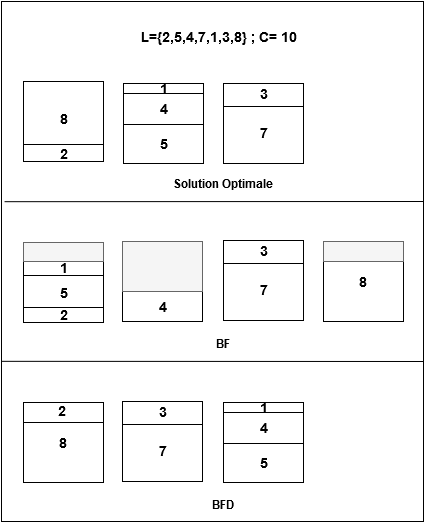
\includegraphics[width=\linewidth]{../figures/BF BFD.png}
    \caption{Exemple BF et BFD}
\end{figure}
\newpage
\end{document}